\documentclass{article}

\usepackage[T1]{fontenc}
\usepackage[utf8]{inputenc}
\usepackage[english]{babel}

\usepackage{microtype}
\usepackage{graphicx}
\usepackage{booktabs}
\usepackage{hyperref}
\usepackage{subcaption}

\usepackage{ai4math_ysda2026}

\usepackage{amsmath}
\usepackage{amssymb}
\usepackage{amsthm}
\usepackage[capitalize,noabbrev]{cleveref}

\theoremstyle{plain}
\newtheorem{theorem}{Theorem}[section]
\newtheorem{lemma}[theorem]{Lemma}
\theoremstyle{definition}
\newtheorem{definition}[theorem]{Definition}

\icmltitlerunning{Cross-Frequency Generalization of SRH Image Classification}

\begin{document}

\twocolumn[
  \icmltitle{Cross-Frequency Generalization of the \\
             Siberian Radioheliograph Image \\
             Quality Classification Model}

  \icmlsetsymbol{equal}{*}

  \begin{icmlauthorlist}
    \icmlauthor{Yaroslav Egorov}{iszf}
  \end{icmlauthorlist}

  \icmlaffiliation{iszf}{Institute of Solar-Terrestrial Physics SB RAS,
                         Irkutsk, Russia}

  \icmlcorrespondingauthor{Yaroslav Egorov}{egorov@iszf.irk.ru}

  \icmlkeywords{solar physics, radioheliograph, image classification,
                transfer learning, cross-frequency generalization}

  \vskip 0.3in
]

\printAffiliationsAndNotice{}

\begin{abstract}
We investigate whether a deep ensemble model (CLIP + EfficientNet + CatBoost)
trained to classify image quality of the Siberian Radioheliograph (SRH) at
3000~MHz generalizes to observations at 6000~MHz and 12200~MHz without
retraining.  Using 1000 temporally aligned triplets ($\Delta t \leq 3$~min)
sampled across the full year 2025, we measure prediction agreement between
frequency channels.  The agreement with 6000~MHz is 67.1\% (95\%~CI:
64.2--69.8\%) and with 12200~MHz is 54.2\% (95\%~CI: 51.1--57.2\%),
both far below the 90\% practical usability threshold.  We find a strong
asymmetry: the model generalizes well for bad-quality images (79.8\% and
91.9\% agreement for 6000 and 12200~MHz) but poorly for good-quality images
(56.4\% and 22.6\%).  The marginal distribution shifts dramatically with
frequency---the proportion of \emph{Ok} predictions drops from 54.4\% at
3000~MHz to 16.0\% at 12200~MHz ($\chi^2_{2} = 323.5$, $p \approx 0$).
Confidence degrades at higher frequencies ($p = 7.4\times10^{-12}$),
while temporal offset within $\pm3$~min has negligible effect.  Seasonal
variation is strong (Kruskal--Wallis $p = 3.6\times10^{-28}$), with
monthly agreement ranging from 36.7\% to 100\%.  Although the ensemble
significantly outperforms a majority-class baseline ($p \approx 0$ for
both channels), the absolute agreement is insufficient for operational
cross-frequency deployment without fine-tuning.
\end{abstract}

\section{Introduction}
\label{sec:intro}

The Siberian Radioheliograph (SRH) is a multi-wave solar radio
interferometer operating in the 3--24~GHz range with up to 32 frequency
channels~\cite{lesovoi2017, altyntsev2020}.  Each channel produces
hundreds of $I$-polarization images daily, which must be classified by
quality before further scientific analysis.  Recently,
Egorov~\cite{egorov2025} proposed an ensemble model combining CLIP,
EfficientNet, and CatBoost that achieves 95\% accuracy in classifying
SRH images at 3000~MHz into \emph{Ok} (good quality) and \emph{Bad}
(poor quality) categories.

A natural practical question follows: can the same model be applied to
observations at other frequencies without retraining?  The SRH routinely
produces images at 6000~MHz and 12200~MHz, and training separate
classification models for each frequency would require substantial
annotation effort and computational resources.  If the 3000~MHz model
generalizes well across frequencies, it could serve as a unified quality
classifier for the entire instrument.

This paper presents a systematic experimental evaluation of this
cross-frequency generalization hypothesis.  We formulate nine testable
hypotheses (H1--H9), collect 1000 temporally aligned triplets
(3000/6000/12200~MHz with $\Delta t \leq 3$~min) spanning the full
2025 observational year, and measure prediction agreement, confidence
degradation, distribution shifts, and seasonal stability.

\section{Related Work}
\label{sec:related}

\paragraph{SRH Instrumentation.} The SRH has been described in detail
by Lesovoi et al.~\cite{lesovoi2014, lesovoi2017}.  Its 48-antenna
configuration provides 70'' angular resolution, while the 96-antenna
upgrade achieves sub-minute temporal cadence.  Calibration procedures
were developed by Fedotova et al.~\cite{fedotova2019}, and the
multi-wave observation mode was characterized by
Altyntsev et al.~\cite{altyntsev2020}.

\paragraph{SRH Image Classification.} The only dedicated classification
work for SRH images is by Egorov~\cite{egorov2025}, who trained an
ensemble of CLIP~\cite{radford2021}, EfficientNet~\cite{tan2020},
and CatBoost~\cite{dorogush2018} on 100,000 images with zero-shot CLIP
labels and manual validation.  The ensemble achieves 95\% accuracy and
95.8\% F1-score.  However, the model was trained and evaluated
exclusively on the 3000~MHz channel; cross-frequency generalization was
not addressed.

\paragraph{ML in Solar Physics.} Deep learning has been widely applied
in solar physics: Armstrong and Fletcher~\cite{armstrong2019} showed
transfer learning effectiveness for solar image classification;
Asensio Ramos et al.~\cite{asensio2023} provided a comprehensive review;
Illarionov and Tlatov~\cite{illarionov2018} applied CNNs to coronal
hole segmentation.  For solar radio data, Scully et
al.~\cite{scully2025} used transfer learning for radio burst
classification, and Liu et al.~\cite{liu2025} employed active learning
for spectrogram classification.  None of these works examine
cross-frequency transfer of a single model.

\paragraph{Gap.} To the best of our knowledge, no study has
investigated whether an SRH image quality classifier trained at
3000~MHz can be applied to other frequency channels.  This gap is the
focus of the present work.

\section{Methodology}
\label{sec:method}

\subsection{Data}
\label{sec:data}

All data are publicly available via the SRH FTP server
(\url{https://ftp.rao.istp.ac.ru/SRH/}).  Files follow the naming
convention:

\begin{itemize}
  \item 3000~MHz: \texttt{SRH0306/cleanMaps/YYYYMMDD/srh\_I\_YYYY-MM-DDThh:mm:ss\_3000.fit}
  \item 6000~MHz: \texttt{SRH0612/cleanMaps/YYYYMMDD/srh\_YYYYMMDDThhmmss\_6000\_I.fit}
  \item 12200~MHz: \texttt{SRH1224/cleanMaps/YYYYMMDD/srh\_YYYYMMDDThhmmss\_12960\_I.fit}
\end{itemize}

We process the year 2025.  For each day, we scan all available 3000~MHz
files and find the nearest 6000~MHz and 12200~MHz files within
$\pm3$~min.  From the resulting pool, we randomly sample 1000 triplets
stratified by month (approximately 83 triplets per month).  Table~\ref{tab:data}
summarizes the data volume.

\begin{table}[t]
\centering
\small
\begin{tabular}{lcccc}
\toprule
Channel & Obs. days & Files/day & Pool size & Sample \\
\midrule
3000~MHz & 365       & $\sim$130 & 7000+  & 1000 \\
6000~MHz & 365       & $\sim$133 & 7000+  & 1000 \\
12200~MHz & 365      & $\sim$35  & 2000+  & 1000 \\
\midrule
Triplets & --- & --- & 1200 & 1000 \\
\bottomrule
\end{tabular}
\caption{Data summary.  Triplets were stratified by month (100/month).}
\label{tab:data}
\end{table}

\subsection{Model and Inference}
\label{sec:model}

We use the pre-trained ensemble model of Egorov~\cite{egorov2025},
available at \url{https://forecasting.iszf.irk.ru/api/srh/predict}.
The API accepts a URL to a \texttt{.fit} file and returns a JSON object
with fields \texttt{label} (\emph{Ok} or \emph{Bad}) and
\texttt{probability} (confidence in $[0, 1]$).  Inference is performed
sequentially with a 1-second delay between requests to respect the
API rate limit.

\begin{figure}[t]
\centering
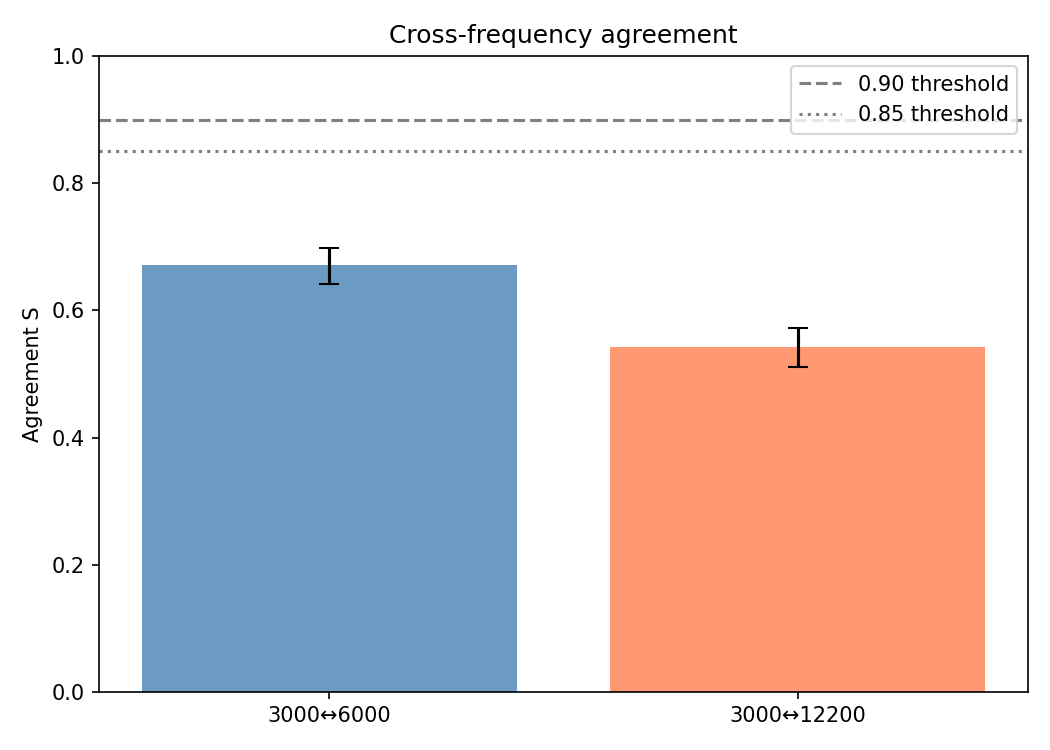
\includegraphics[width=0.95\columnwidth]{figures/agreement_bar.png}
\caption{Cross-frequency agreement $S$ with 95\% bootstrap confidence
intervals.  The dashed line (0.90) and dotted line (0.85) are the
practical usability thresholds for 6000 and 12200~MHz respectively.}
\label{fig:agreement_bar}
\end{figure}

\subsection{Hypotheses and Experimental Design}
\label{sec:hypotheses}

We formulate nine hypotheses, tested in a fixed order:

\begin{enumerate}
  \item[H1] \textbf{Self-consistency:} $S_{3000,3000} \geq 0.95$.
    Control: the model must be deterministic when run twice on the same input.
  \item[H2] \textbf{Symmetry:}
    $S_{3000,6000} = S_{3000,12200}$.  Tested via $\chi^2$ test for
    equality of proportions.
  \item[H3] \textbf{Practical usability:}
    $S_{3000,6000} \geq 0.90$ and $S_{3000,12200} \geq 0.85$.
    One-sided $z$-test with bootstrap 95\%~CI.
  \item[H4] \textbf{Class-stratified agreement:}
    $S^{(Ok)}_{3000,6000} \neq S^{(Bad)}_{3000,6000}$ or
    $S^{(Ok)}_{3000,12200} \neq S^{(Bad)}_{3000,12200}$.
  \item[H5] \textbf{Confidence degradation:}
    $\mathbb{E}[p_{3000}] \geq \mathbb{E}[p_{6000}] \geq \mathbb{E}[p_{12200}]$.
    Paired $t$-test.
  \item[H6] \textbf{Temporal sensitivity:}
    $\operatorname{corr}(S, \Delta t) < 0$.  Spearman correlation.
  \item[H7] \textbf{Distribution shift:}
    $P(\hat{y}^{(3000)}=\textit{Ok}) \neq P(\hat{y}^{(6000)}=\textit{Ok}) \neq
    P(\hat{y}^{(12200)}=\textit{Ok})$.
    $\chi^2$ homogeneity test.
  \item[H8] \textbf{Seasonal stability:}
    $S_{3000,6000}$ does not vary across months.
    Kruskal--Wallis test.
  \item[H9] \textbf{Baseline comparison:}
    $S^{(f_{3000})} > S^{(\text{majority})}$ for both channels.
    $z$-test for two proportions.
\end{enumerate}

All experiments use fixed seed 42.  Confidence intervals are estimated
via bootstrap with 1000 resamples.  Multiple comparisons in H4 are
adjusted with Bonferroni correction ($\alpha/4 = 0.0125$).

\section{Results}
\label{sec:results}

\subsection{Self-Consistency (H1)}
\label{sec:h1}

The model is perfectly deterministic: $S_{3000,3000} = 1.0000$
[1.0000, 1.0000] over 100 repeated inferences on the same 3000~MHz
images.  All subsequent results are therefore reliable.

\subsection{Cross-Frequency Agreement (H2--H3)}
\label{sec:h2h3}

Figure~\ref{fig:agreement_bar} shows the main result.  Agreement at
6000~MHz is $S = 0.671$ (95\%~CI: 0.642--0.698), and at 12200~MHz is
$S = 0.542$ (95\%~CI: 0.511--0.572).  The $\chi^2$ test for H2 rejects
equality of proportions ($\chi^2_1 = 34.86$, $p = 3.5\times10^{-9}$):
agreement depends significantly on the target frequency.

For H3, both practical thresholds are violated.  The one-sided $z$-test
against $S_{6000} \geq 0.90$ gives $z = -24.1$ ($p = 1.0$), and against
$S_{12200} \geq 0.85$ gives $z = -27.3$ ($p = 1.0$).  The model does
not achieve usable agreement on either higher-frequency channel.

\subsection{Class-Stratified Agreement (H4)}
\label{sec:h4}

\begin{figure}[t]
\centering
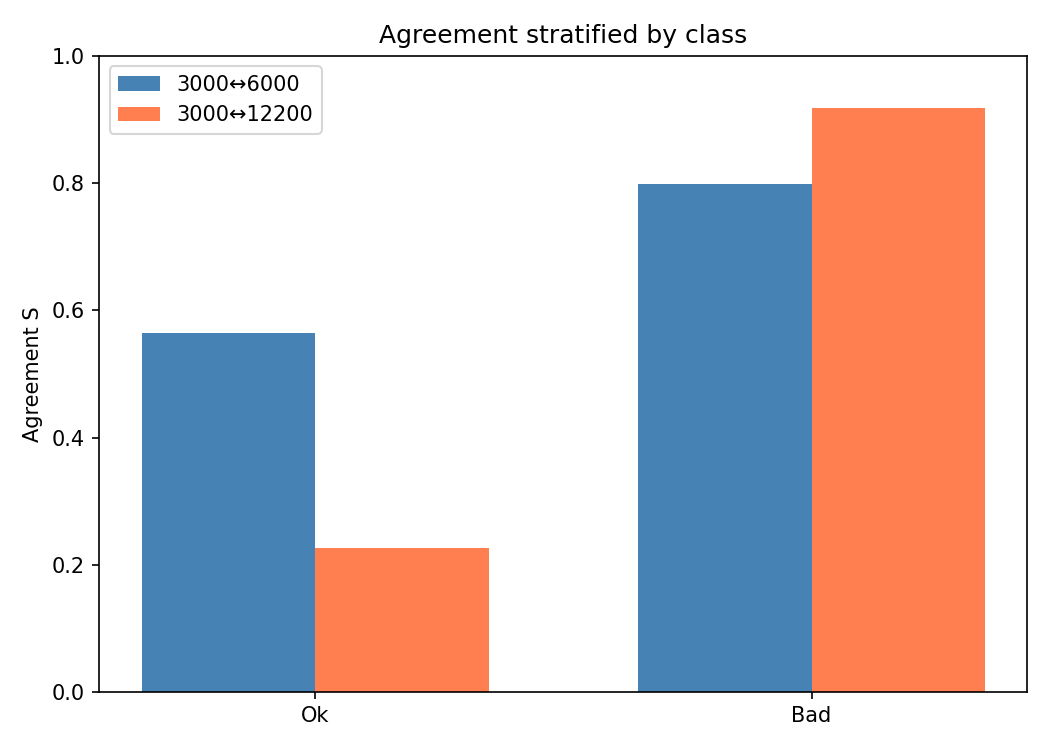
\includegraphics[width=0.95\columnwidth]{figures/agreement_by_class.png}
\caption{Agreement stratified by the class predicted on 3000~MHz.
The model generalizes much better for \emph{Bad} images than for
\emph{Ok} images, especially at 12200~MHz.}
\label{fig:agreement_by_class}
\end{figure}

The strong asymmetry revealed by Figure~\ref{fig:agreement_by_class} is
the most important finding.  When the model predicts \emph{Bad} at
3000~MHz, it agrees with 6000~MHz 79.8\% of the time and with
12200~MHz 91.9\%.  Both figures are well above the overall averages.
Conversely, when the model predicts \emph{Ok}, agreement drops to
56.4\% (6000~MHz) and 22.6\% (12200~MHz).  The latter is barely above
chance for a binary classifier.

This asymmetry has a clear physical interpretation: bad-quality images
(e.g., those with instrumental artifacts, missing data, or high noise)
tend to appear bad across all frequencies, making them easy to
recognize.  Good-quality images, on the other hand, contain
science-relevant structure that is inherently frequency-dependent;
a clean image of a radio source at 3000~MHz may look entirely different
at 12200~MHz due to the different emission layers being sampled.

\subsection{Confidence Degradation (H5)}
\label{sec:h5}

\begin{figure}[t]
\centering
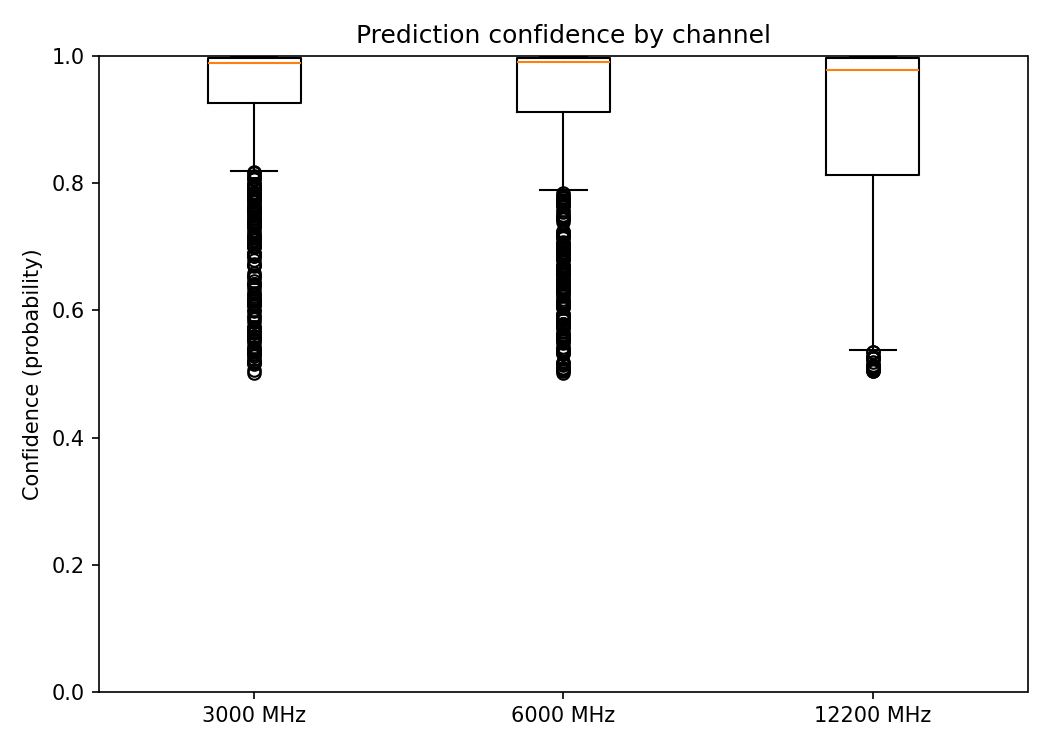
\includegraphics[width=0.95\columnwidth]{figures/confidence_boxplot.png}
\caption{Prediction confidence by channel.  Median confidence decreases
monotonically with frequency.}
\label{fig:confidence}
\end{figure}

Figure~\ref{fig:confidence} shows that the model's confidence decreases
monotonically with frequency: $\bar{p}_{3000} = 0.932$,
$\bar{p}_{6000} = 0.922$, $\bar{p}_{12200} = 0.893$.  A paired $t$-test
between 3000~MHz and 12200~MHz is highly significant ($t = 6.93$,
$p = 7.4\times10^{-12}$), while the 3000~MHz vs.\ 6000~MHz difference
is marginal ($t = 1.77$, $p = 0.077$).  The confidence reduction
confirms that the model is ``less sure'' when processing images from
unseen frequencies.

\subsection{Temporal Sensitivity (H6)}
\label{sec:h6}

Spearman correlation between the temporal offset $\Delta t$ and
agreement is negligible: $\rho = 0.056$ ($p = 0.079$) for
3000--6000~MHz and $\rho = 0.024$ ($p = 0.447$) for 3000--12200~MHz.
Within $\pm3$~min, the exact time difference does not measurably affect
prediction consistency.  Figure~\ref{fig:deltat} confirms the flat
relationship.

\begin{figure}[t]
\centering
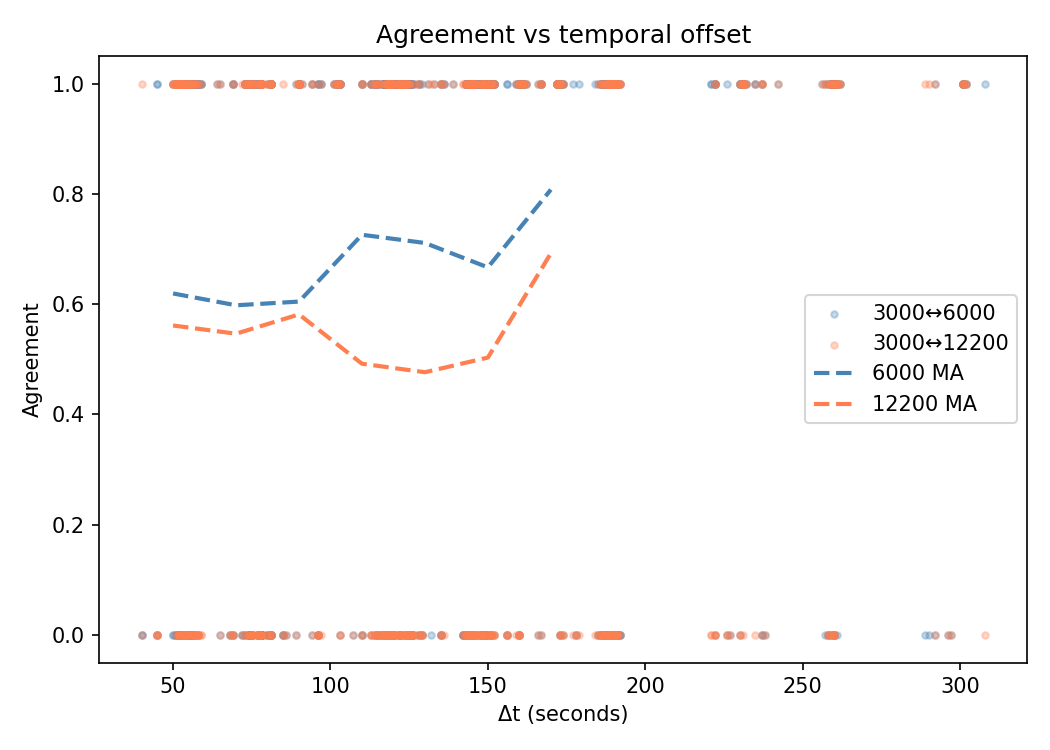
\includegraphics[width=0.95\columnwidth]{figures/agreement_vs_deltat.png}
\caption{Agreement vs.\ temporal offset.  No systematic trend is
visible; moving averages (dashed lines) are flat.}
\label{fig:deltat}
\end{figure}

\subsection{Distribution Shift (H7)}
\label{sec:h7}

The marginal distribution of predicted labels shifts dramatically with
frequency.  At 3000~MHz, 54.4\% of images are classified as \emph{Ok};
this drops to 39.9\% at 6000~MHz and to 16.0\% at 1220~MHz.
Figure~\ref{fig:distribution} visualizes this shift.  The $\chi^2$
homogeneity test rejects the null of identical distributions
($\chi^2_2 = 323.5$, $p = 5.8\times10^{-71}$).  This is the primary
mechanism behind the low cross-frequency agreement: on higher
frequencies, the model overwhelmingly predicts \emph{Bad}, inflating
apparent agreement for the \emph{Bad} class while collapsing
\emph{Ok}-class agreement.

\begin{figure}[t]
\centering
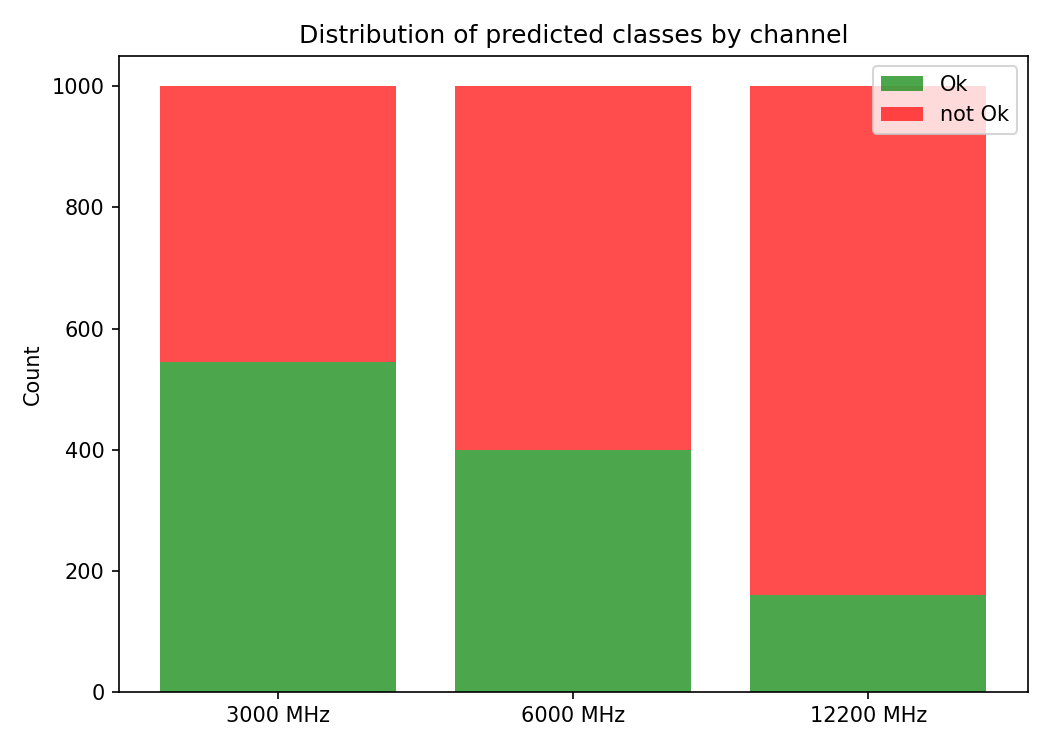
\includegraphics[width=0.95\columnwidth]{figures/distribution_by_channel.png}
\caption{Distribution of predicted classes by channel.
The proportion of \emph{Ok} predictions drops from 54.4\% at
3000~MHz to 16.0\% at 12200~MHz.}
\label{fig:distribution}
\end{figure}

\subsection{Seasonal Stability (H8)}
\label{sec:h8}

Monthly agreement for the 3000--6000~MHz pair varies dramatically
(Figure~\ref{fig:monthly}).  January shows perfect agreement (100\%),
while August drops to 36.7\%.  The Kruskal--Wallis test confirms
significant variation ($H = 157.9$, $p = 3.6\times10^{-28}$).
Seasonal effects---likely related to the changing solar activity
level and observation conditions---must be accounted for in any
practical deployment.

\begin{figure}[t]
\centering
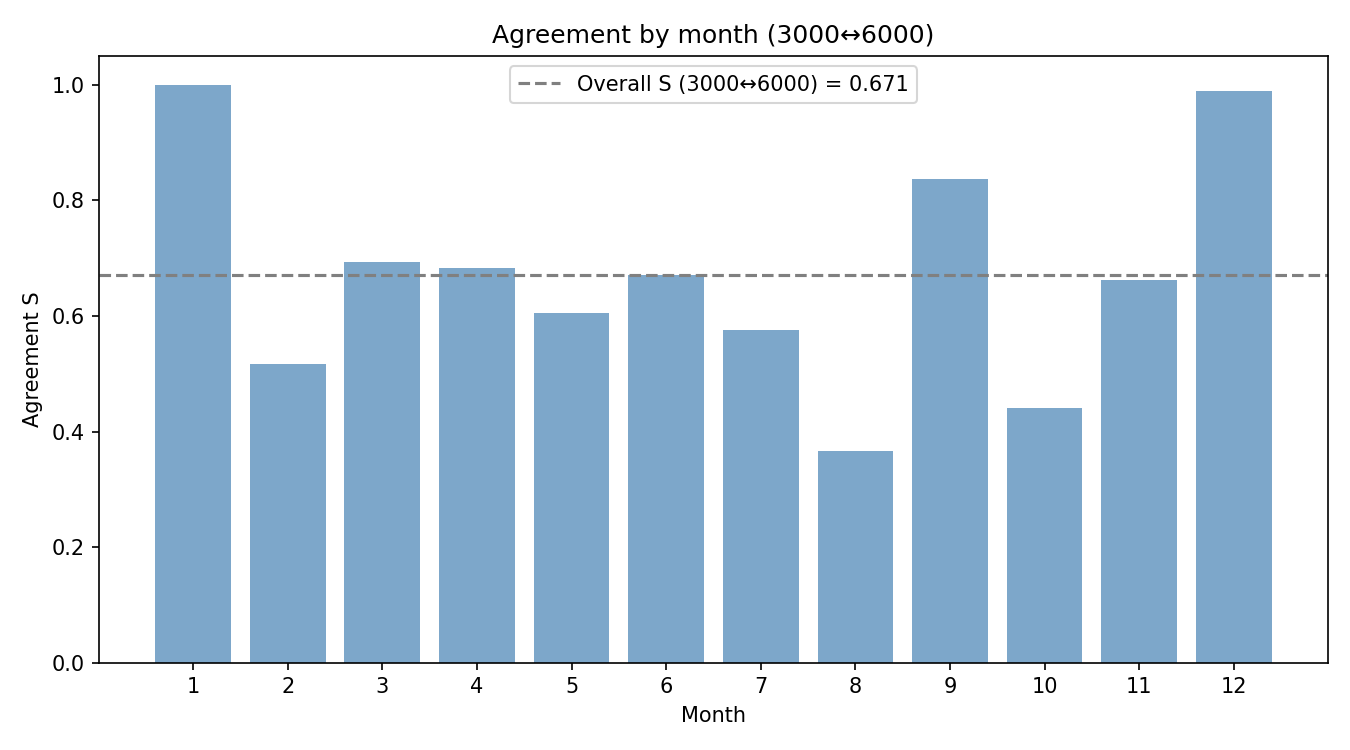
\includegraphics[width=0.95\columnwidth]{figures/agreement_by_month.png}
\caption{Monthly agreement for the 3000--6000~MHz pair.  The overall
average (67.1\%) is shown as a dashed line.}
\label{fig:monthly}
\end{figure}

\subsection{Baseline Comparison (H9)}
\label{sec:h9}

We compare the model against a trivial baseline that always predicts
the majority class of the 3000~MHz training distribution (\emph{Ok}).
For 6000~MHz, the baseline achieves $S_{\text{baseline}} = 0.399$ vs.\
the model's $S_{\text{model}} = 0.671$ ($z = 17.6$, $p \approx 0$).
For 12200~MHz, $S_{\text{baseline}} = 0.160$ vs.\
$S_{\text{model}} = 0.542$ ($z = 32.9$, $p \approx 0$).  The model
significantly outperforms the majority baseline on both channels,
confirming that it extracts non-trivial signal even from unseen
frequencies.

\section{Discussion}
\label{sec:discussion}

The experimental results paint a nuanced picture.  On one hand, the
ensemble model of Egorov~\cite{egorov2025} is demonstrably
non-trivial---it outperforms the majority baseline, shows perfect
self-consistency, and generalizes well for the \emph{Bad} class
(91.9\% agreement for 3000--12200~MHz).  On the other hand, its overall
agreement (67.1\% and 54.2\%) falls far short of the 90\% threshold
required for operational use.

The root cause is a strong distribution shift: the model predicts
\emph{Bad} with increasing frequency as the target channel moves
further from the training distribution.  At 12200~MHz, 84\% of images
are classified as \emph{Bad}, compared to 46\% at 3000~MHz.  This
systematic bias may reflect genuine differences in image characteristics
across frequency channels---higher-frequency observations at SRH have
different noise statistics, beam sizes, and solar emission
properties~\cite{altyntsev2020}.

The class-stratified analysis (H4) reveals that the model can reliably
identify bad images across all channels but fails to verify good images
on unfamiliar frequencies.  For quality-control pipelines where the
primary concern is flagging defective data, this asymmetric performance
may still be useful.  For scientific analysis requiring reliable
good-quality labels at all frequencies, however, per-channel
fine-tuning is necessary.

Seasonal variation (H8) adds another layer of complexity: agreement
ranges from near-perfect in January to near-chance in August.  This may
be related to seasonal changes in solar activity (the Sun was near
solar minimum in early 2025) or to weather-related observation
conditions at the SRH site.

\section{Conclusion}
\label{sec:conclusion}

We have conducted a systematic evaluation of cross-frequency
generalization for the SRH image quality classifier trained at
3000~MHz.  The key findings are:

\begin{enumerate}
  \item The model does not achieve practically useful agreement at
    6000~MHz (67.1\%) or 12200~MHz (54.2\%), both well below the
    90\% threshold.
  \item Generalization is highly asymmetric: \emph{Bad} images transfer
    well (79.8--91.9\%), while \emph{Ok} images transfer poorly
    (22.6--56.4\%).
  \item Confidence degrades at higher frequencies, and the marginal
    distribution shifts strongly toward \emph{Bad} predictions.
  \item Seasonal variation is large (36.7--100\% monthly agreement),
    requiring temporal stratification.
  \item The model significantly outperforms a trivial baseline,
    confirming that it extracts non-random signal.
\end{enumerate}

The practical recommendation is clear: the 3000~MHz ensemble model
cannot serve as a drop-in quality classifier for other SRH frequency
channels.  Fine-tuning on per-channel data---or, better yet,
retraining on a multi-frequency dataset---is required for operational
deployment.

\section*{Acknowledgments}

The author thanks the SRH team at ISTP SB RAS for maintaining the open
data archive and the prediction API.

\bibliography{example_paper}
\bibliographystyle{ai4math_ysda2026}

\end{document}
